\documentclass[7pt,landscape]{extarticle}
\usepackage[margin=0.12in]{geometry}
\usepackage{multicol}
\usepackage{amsmath,amssymb}
\usepackage{enumitem}
\usepackage{titlesec}
\usepackage{booktabs}
\usepackage{graphicx}
\usepackage{xcolor}
\usepackage{tikz}
\usetikzlibrary{arrows.meta, positioning, calc, patterns}

\setlength{\parindent}{0pt}
\setlength{\parskip}{0.15em}
\setlist{nosep, leftmargin=*, topsep=0pt, partopsep=0pt}
\titlespacing*{\section}{0pt}{2pt}{0.5pt}
\titlespacing*{\subsection}{0pt}{1.5pt}{0pt}

\titleformat{\section}{\bfseries\fontsize{7.5}{8.5}\selectfont\color{blue}}{}{0em}{}
\titleformat{\subsection}{\bfseries\fontsize{6.5}{7.5}\selectfont\color{teal}}{}{0em}{}

\tikzset{
    axis/.style={->, >=stealth, thin},
    curve/.style={thick, smooth},
    dashed_line/.style={dashed, thin, gray},
    every node/.style={font=\tiny}
}

\begin{document}
\fontsize{6.5}{7.5}\selectfont
\begin{multicols*}{4}

%========== WEEK 1 ==========
\section*{Week 1: Intro}
\vspace{-2pt}
\begin{center}
\scalebox{0.38}{
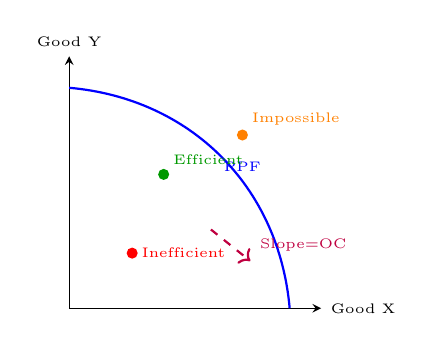
\begin{tikzpicture}[baseline]
    % PPF Diagram
    \draw[axis] (0,0) -- (3.2,0) node[right] {Good X};
    \draw[axis] (0,0) -- (0,3.2) node[above] {Good Y};
    \draw[curve, blue] (0,2.8) to[out=-5, in=95] (2.8,0);
    \node[blue] at (2.2, 1.8) {PPF};
    \fill[red] (0.8,0.7) circle (2pt) node[right, red] {Inefficient};
    \fill[green!60!black] (1.2, 1.7) circle (2pt) node[above right, green!60!black] {Efficient};
    \fill[orange] (2.2, 2.2) circle (2pt) node[above right, orange] {Impossible};
    \draw[->, thick, purple, dashed] (1.8,1.0) -- (2.3,0.6);
    \node[purple, anchor=west] at (2.3,0.8) {Slope=OC};
\end{tikzpicture}
}
\end{center}
\vspace{-5pt}

\subsection*{Core Concepts}
\begin{itemize}
    \item \textbf{Scarcity}: Resources limited, wants unlimited $\implies$ must choose.
    \item \textbf{Opportunity Cost}: Value of \textit{best alternative forgone}. ``No free lunch.''
    \item E.g. Med school = Tuition + Books + \textbf{Forgone Earnings}.
    \item E.g. ``Free'' vaccine clinic: OC of time (travel + wait).
    \item \textbf{Marginal Thinking}: Decide on the \textit{next} unit. If $MB > MC$, do it; if $MB < MC$, stop. Optimal: $MB = MC$.
    \item \textbf{Sunk Costs}: Irrelevant to future decisions.
    \item \textbf{Rationality}: 1. Complete; 2. Transitive ($A>B, B>C \Rightarrow A>C$); 3. Respond to Incentives.
    \item \textbf{Positive}: ``What is?'' Testable. \textbf{Normative}: ``What should be?'' Value judgment.
\end{itemize}

\subsection*{8 Factors of Health Econ}
\begin{enumerate}[leftmargin=1.2em]
    \item \textbf{Derived Demand}: Want health, not care itself.
    \item \textbf{Uncertainty}: When sick? Treatment works?
    \item \textbf{Gov't Involvement}: Largest payer \& regulator.
    \item \textbf{Externalities}: Vaccination $\to$ herd immunity.
    \item \textbf{Non-profit Firms}: Many hospitals non-profit.
    \item \textbf{Equity}: Fairness in resource distribution.
    \item \textbf{Asymmetric Info}: Dr knows more $\to$ principal-agent; weakens ``shopping''.
    \item \textbf{Insurance}: Effective price $\ll$ true cost $\to$ moral hazard.
\end{enumerate}

\subsection*{PPF (Production Possibility Frontier)}
\begin{itemize}
    \item On curve = Efficient; Inside = Inefficient; Outside = Impossible.
    \item Slope = OC ($MRT$). Concave (bowed out) due to specialization.
    \item Shifts outward: tech progress or resource growth.
\end{itemize}

%========== WEEK 2 ==========
\section*{Week 2: Demand}
\vspace{-2pt}
\begin{center}
\scalebox{0.38}{
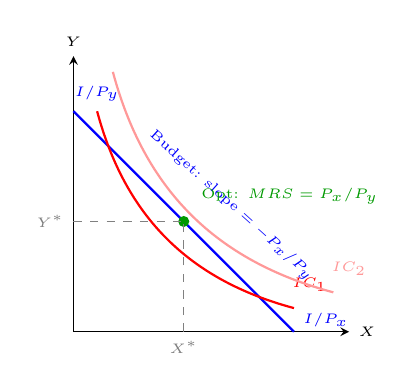
\begin{tikzpicture}[baseline]
    % IC + Budget Constraint
    \draw[axis] (0,0) -- (3.5,0) node[right] {$X$};
    \draw[axis] (0,0) -- (0,3.5) node[above] {$Y$};
    % Budget line
    \draw[thick, blue] (0,2.8) -- (2.8,0);
    \node[blue, anchor=south] at (0.3,2.8) {$I/P_y$};
    \node[blue, anchor=west] at (2.8,0.15) {$I/P_x$};
    \node[blue, rotate=-42] at (2.0, 1.6) {Budget: slope $= -P_x/P_y$};
    % IC curves
    \draw[curve, red] (0.3,2.8) to[out=-75, in=165] (2.8,0.3);
    \node[red] at (3.0,0.6) {$IC_1$};
    \draw[curve, red!40] (0.5,3.3) to[out=-75, in=165] (3.3,0.5);
    \node[red!40] at (3.5,0.8) {$IC_2$};
    % Tangency
    \fill[green!60!black] (1.4, 1.4) circle (2pt);
    \node[green!60!black, anchor=south west] at (1.5, 1.5) {Opt: $MRS = P_x/P_y$};
    \draw[dashed_line] (1.4,0) -- (1.4,1.4) node[below, at start] {$X^*$};
    \draw[dashed_line] (0,1.4) -- (1.4,1.4) node[left, at start] {$Y^*$};
\end{tikzpicture}
}
\end{center}
\vspace{-5pt}

\subsection*{Utility \& Consumer Choice}
\begin{itemize}
    \item \textbf{Utility}: Satisfaction. \textbf{Diminishing MU}: Extra unit $\to$ less satisfaction.
    \item \textbf{Demand Curve} = WTP = Marginal Benefit curve.
    \item \textbf{IC}: Same-utility bundles. Downward sloping, Convex, Never cross. Far = higher $U$.
    \item \textbf{MRS} = $|$Slope of IC$|$ = $MU_x/MU_y$. Diminishing.
    \item \textbf{Budget}: $I = P_x X + P_y Y$. Slope $= -P_x/P_y$.
    \item \textbf{Optimum}: Tangency. $MRS_{xy} = \frac{P_x}{P_y} \iff \frac{MU_x}{P_x} = \frac{MU_y}{P_y}$ (equal ``bang per buck'').
\end{itemize}

\subsection*{Grossman Model}
\vspace{-2pt}
\begin{center}
\scalebox{0.38}{
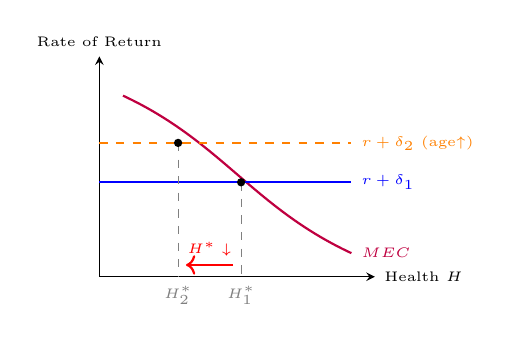
\begin{tikzpicture}[baseline]
    \draw[axis] (0,0) -- (3.5,0) node[right] {Health $H$};
    \draw[axis] (0,0) -- (0,2.8) node[above] {Rate of Return};
    % MEC curve
    \draw[curve, purple] (0.3,2.3) to[out=-25, in=155] (3.2,0.3) node[right] {$MEC$};
    % r+delta lines
    \draw[thick, blue] (0,1.2) -- (3.2,1.2) node[right] {$r+\delta_1$};
    \draw[thick, orange, dashed] (0,1.7) -- (3.2,1.7) node[right] {$r+\delta_2$ (age$\uparrow$)};
    % Optimal points
    \draw[dashed_line] (1.8,1.2) -- (1.8,0) node[below] {$H_1^*$};
    \draw[dashed_line] (1.0,1.7) -- (1.0,0) node[below] {$H_2^*$};
    \fill (1.8,1.2) circle (1.5pt);
    \fill (1.0,1.7) circle (1.5pt);
    \draw[->, thick, red] (1.7,0.15) -- (1.1,0.15);
    \node[red] at (1.4, 0.35) {$H^*\downarrow$};
\end{tikzpicture}
}
\end{center}
\vspace{-5pt}
\begin{itemize}
    \item People demand \textbf{Health}, not care. Care is \textbf{derived demand}.
    \item Health: 1. \textbf{Consumption good} (feel good); 2. \textbf{Investment good} (healthy time $h_t$).
    \item $H_t = H_{t-1}(1-\delta) + I_{t-1}$. Optimal: $MEC = r + \delta$.
    \item Age $\uparrow \to \delta \uparrow \to H^* \downarrow$. Wage/Edu $\uparrow \to MEC$ right $\to H^* \uparrow$.
\end{itemize}

\subsection*{Demand Shifters}
\vspace{-2pt}
\begin{center}
\scalebox{0.38}{
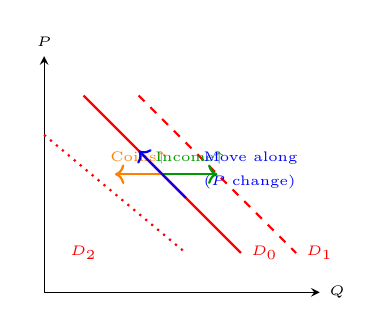
\begin{tikzpicture}[baseline]
    \draw[axis] (0,0) -- (3.5,0) node[right] {$Q$};
    \draw[axis] (0,0) -- (0,3) node[above] {$P$};
    % Original demand
    \draw[thick, red] (0.5,2.5) -- (2.5,0.5) node[right] {$D_0$};
    % Shifted demand right
    \draw[thick, red, dashed] (1.2,2.5) -- (3.2,0.5) node[right] {$D_1$};
    % Shifted demand left
    \draw[thick, red, dotted] (0,2.0) -- (1.8,0.5);
    \node[red] at (0.5, 0.5) {$D_2$};
    % Arrow for shift
    \draw[->, thick, green!60!black] (1.5,1.5) -- (2.2,1.5) node[midway, above] {Income$\uparrow$};
    \draw[->, thick, orange] (1.5,1.5) -- (0.9,1.5) node[midway, above] {Coins$\uparrow$};
    % Movement along
    \draw[->, thick, blue] (1.8,1.2) -- (1.2,1.8);
    \node[blue, anchor=west] at (1.9,1.7) {Move along};
    \node[blue, anchor=west] at (1.9,1.4) {($P$ change)};
\end{tikzpicture}
}
\end{center}
\vspace{-5pt}
\textbf{Move along}: Only own-price change.\\
\textbf{Shift}: Non-price factors:
\begin{enumerate}[leftmargin=1.2em]
    \item \textbf{Income} $\uparrow$: Normal good $\to$ D Right.
    \item \textbf{Related prices}: Sub $P\uparrow \to$ D Right; Comp $P\uparrow \to$ D Left.
    \item \textbf{Tastes}. 4. \textbf{Expectations}. 5. \textbf{\# Buyers}.
\end{enumerate}
\textbf{Coinsurance} $\uparrow$: OOP price $\uparrow \to$ D Left (provider-price axis) or move along (OOP axis). \textbf{Draw graph!}

\subsection*{Elasticity}
\textbf{Own-Price}: $E_d = \frac{\%\Delta Q}{\%\Delta P}$.

\begin{tabular}{@{}lll@{}}
$|E|>1$ & Elastic & $P\uparrow \Rightarrow TR\downarrow$ \\
$|E|<1$ & Inelastic & $P\uparrow \Rightarrow TR\uparrow$ \\
$|E|=1$ & Unit & $TR$ max/unchanged \\
\end{tabular}

\textbf{Cross}: $E_{xy} = \frac{\%\Delta Q_x}{\%\Delta P_y}$. $>0$ Subs; $<0$ Comps.

\textbf{Income}: $E_I = \frac{\%\Delta Q}{\%\Delta I}$. $<0$ Inferior; $0{-}1$ Necessity; $>1$ Luxury.

\textbf{Indiv vs Market}: Single firm $|E_d|$ HIGH (subs exist); whole category $|E_d|$ LOW (no subs, necessity).

\subsection*{TR Test Calculation}
$TR_{new} = (1+\%\Delta P)(1 + E_d \cdot \%\Delta P) \cdot TR_{old}$\\
E.g. $\%\Delta P = 15\%$, $E_d = -0.12$: $TR_{new} = 1.15 \times 0.982 = 1.129 \cdot TR$ ($\uparrow 12.9\%$).\\
E.g. $E_d = -1.6$: $TR_{new} = 1.15 \times 0.76 = 0.874 \cdot TR$ ($\downarrow 12.6\%$).

\subsection*{Moral Hazard \& RAND}
\begin{itemize}
    \item \textbf{Ex-ante}: Less prevention (insured $\to$ less careful).
    \item \textbf{Ex-post}: More care use (OOP price low).
    \item \textbf{RAND HIE}: RCT. $E_d \approx -0.2$ (inelastic but $\neq 0$). Higher copay $\to$ less use. Poor/sick harmed by high cost-sharing.
\end{itemize}

%========== WEEK 3 ==========
\section*{Week 3: Supply}
\vspace{-2pt}
\begin{center}
\scalebox{0.38}{
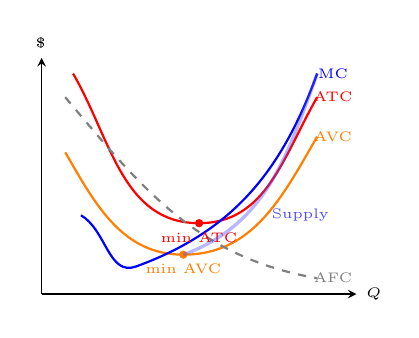
\begin{tikzpicture}[baseline]
    % Cost Curves
    \draw[axis] (0,0) -- (4,0) node[right] {$Q$};
    \draw[axis] (0,0) -- (0,3) node[above] {\$};
    % ATC
    \draw[curve, red] (0.4,2.8) to[out=-60, in=180] (2.0,0.9) to[out=0, in=240] (3.5,2.5);
    \node[red] at (3.7,2.5) {ATC};
    % AVC
    \draw[curve, orange] (0.3,1.8) to[out=-60, in=180] (1.8,0.5) to[out=0, in=240] (3.5,2.0);
    \node[orange] at (3.7,2.0) {AVC};
    % MC
    \draw[curve, blue] (0.5,1.0) to[out=-30, in=200] (1.2,0.35) to[out=20, in=250] (3.5,2.8);
    \node[blue] at (3.7,2.8) {MC};
    % AFC (dashed)
    \draw[curve, gray, dashed] (0.3,2.5) to[out=-50, in=170] (3.5,0.2);
    \node[gray] at (3.7,0.2) {AFC};
    % Min points
    \fill[red] (2.0,0.9) circle (1.5pt) node[below, red] {min ATC};
    \fill[orange] (1.8,0.5) circle (1.5pt) node[below, orange] {min AVC};
    % Supply curve annotation
    \draw[very thick, blue!70, opacity=0.4] (1.8,0.5) to[out=20, in=250] (3.5,2.8);
    \node[blue!70, anchor=west] at (2.8,1.0) {Supply};
\end{tikzpicture}
}
\end{center}
\vspace{-5pt}

\begin{center}
\scalebox{0.38}{
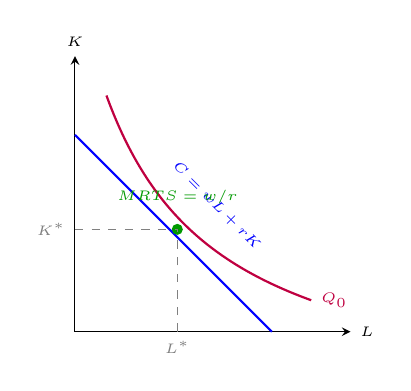
\begin{tikzpicture}[baseline]
    % Isoquant + Isocost
    \draw[axis] (0,0) -- (3.5,0) node[right] {$L$};
    \draw[axis] (0,0) -- (0,3.5) node[above] {$K$};
    % Isoquant
    \draw[curve, purple] (0.4,3.0) to[out=-70, in=160] (3.0,0.4) node[right] {$Q_0$};
    % Isocost
    \draw[thick, blue] (0,2.5) -- (2.5,0);
    \node[blue, rotate=-45] at (1.8,1.6) {$C = wL + rK$};
    % Tangency
    \fill[green!60!black] (1.3,1.3) circle (2pt);
    \node[green!60!black, anchor=south] at (1.3,1.5) {$MRTS = w/r$};
    \draw[dashed_line] (1.3,0) -- (1.3,1.3) node[below, at start] {$L^*$};
    \draw[dashed_line] (0,1.3) -- (1.3,1.3) node[left, at start] {$K^*$};
\end{tikzpicture}
}
\end{center}
\vspace{-5pt}

\subsection*{Production $Q = f(L,K)$}
\begin{itemize}
    \item \textbf{Short Run}: $K$ fixed. \textbf{Long Run}: All variable.
    \item $MP_L = \partial Q / \partial L$. \textbf{Diminishing MP}: $MP_L \downarrow$ as $L \uparrow$.
    \item $AP_L = Q / L$. \textbf{Key}: $MP$ crosses $AP$ at $AP$'s \textbf{max}.
    \item $MP > AP \Rightarrow AP\uparrow$; $MP < AP \Rightarrow AP\downarrow$; $MP = AP \Rightarrow AP$ max.
    \item \textbf{Cobb-Douglas} $Q = AK^\alpha L^\beta$: $MP_L = \beta Q/L$, $MP_K = \alpha Q/K$.
    \item \textbf{Isoquant}: Same-$Q$ combos. Slope $= -MP_L/MP_K$.
    \item \textbf{Isocost}: $C = wL + rK$. Slope $= -w/r$.
    \item \textbf{Optimal}: $\frac{MP_L}{MP_K} = \frac{w}{r} \iff \frac{MP_L}{w} = \frac{MP_K}{r}$.
    \item \textbf{RTS}: $\alpha{+}\beta > 1$ IRS; $=1$ CRS; $<1$ DRS.
\end{itemize}

\subsection*{Costs}
\begin{itemize}
    \item $TC = TFC + TVC$. $ATC = AFC + AVC$.
    \item $AFC \to 0$ as $Q\uparrow$, so $ATC \to AVC$.
    \item $MC = \Delta TVC/\Delta Q = w/MP_L$. \textbf{MC $\propto 1/MP_L$}.
    \item MC crosses ATC \& AVC at their \textbf{min}.
    \item \textbf{Supply} = MC above min AVC (shutdown).
    \item $MR = MC$ (profit max). Perfect comp: $P = MC$.
\end{itemize}

%========== WEEK 4 ==========
\section*{Week 4: Markets}
\vspace{-2pt}
\begin{center}
\scalebox{0.38}{
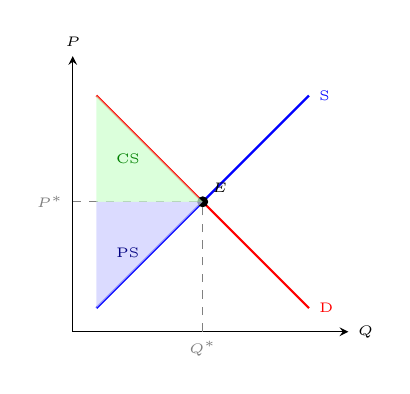
\begin{tikzpicture}[baseline]
    % Market Eq with CS/PS
    \draw[axis] (0,0) -- (3.5,0) node[right] {$Q$};
    \draw[axis] (0,0) -- (0,3.5) node[above] {$P$};
    % S and D
    \draw[thick, blue] (0.3,0.3) -- (3.0,3.0) node[right] {S};
    \draw[thick, red] (0.3,3.0) -- (3.0,0.3) node[right] {D};
    % Equilibrium
    \fill (1.65,1.65) circle (2pt) node[above right] {$E$};
    \draw[dashed_line] (1.65,0) -- (1.65,1.65) node[below, at start] {$Q^*$};
    \draw[dashed_line] (0,1.65) -- (1.65,1.65) node[left, at start] {$P^*$};
    % CS shading
    \fill[green!20, opacity=0.7] (0.3,3.0) -- (1.65,1.65) -- (0.3,1.65) -- cycle;
    \node[green!50!black] at (0.7,2.2) {CS};
    % PS shading
    \fill[blue!20, opacity=0.7] (0.3,0.3) -- (1.65,1.65) -- (0.3,1.65) -- cycle;
    \node[blue!50!black] at (0.7,1.0) {PS};
\end{tikzpicture}
}
\end{center}
\vspace{-5pt}

\begin{center}
\scalebox{0.35}{
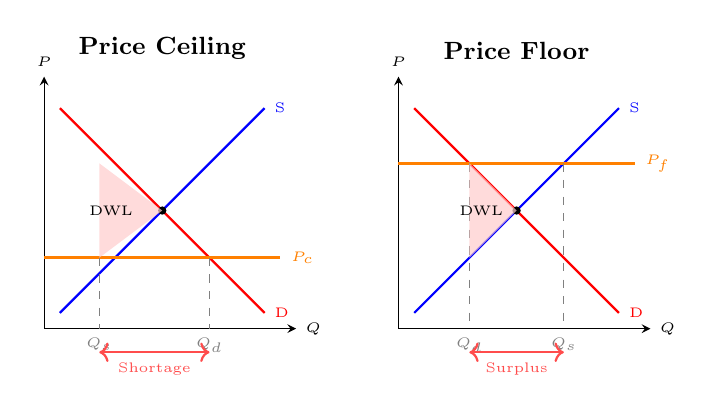
\begin{tikzpicture}[baseline]
    % Price Ceiling (left) and Price Floor (right) side by side
    % === PRICE CEILING ===
    \draw[axis] (0,0) -- (3.2,0) node[right] {$Q$};
    \draw[axis] (0,0) -- (0,3.2) node[above] {$P$};
    \draw[thick, blue] (0.2,0.2) -- (2.8,2.8) node[right] {S};
    \draw[thick, red] (0.2,2.8) -- (2.8,0.2) node[right] {D};
    % Ceiling line
    \draw[very thick, orange] (0,0.9) -- (3.0,0.9) node[right] {$P_c$};
    \fill (1.5,1.5) circle (1.5pt);
    % Qs and Qd at ceiling
    \draw[dashed_line] (0.7,0.9) -- (0.7,0) node[below] {$Q_s$};
    \draw[dashed_line] (2.1,0.9) -- (2.1,0) node[below] {$Q_d$};
    % Shortage
    \draw[<->, thick, red!70] (0.7,-0.3) -- (2.1,-0.3) node[midway, below] {Shortage};
    % DWL
    \fill[red!20, opacity=0.7] (1.5,1.5) -- (0.7,0.9) -- (0.7,2.1) -- cycle;
    \node at (0.85,1.5) {DWL};
    \node[anchor=south, font=\small\bfseries] at (1.5,3.3) {Price Ceiling};
    %
    % === PRICE FLOOR ===
    \begin{scope}[xshift=4.5cm]
    \draw[axis] (0,0) -- (3.2,0) node[right] {$Q$};
    \draw[axis] (0,0) -- (0,3.2) node[above] {$P$};
    \draw[thick, blue] (0.2,0.2) -- (2.8,2.8) node[right] {S};
    \draw[thick, red] (0.2,2.8) -- (2.8,0.2) node[right] {D};
    % Floor line
    \draw[very thick, orange] (0,2.1) -- (3.0,2.1) node[right] {$P_f$};
    \fill (1.5,1.5) circle (1.5pt);
    % Qs and Qd at floor
    \draw[dashed_line] (0.9,2.1) -- (0.9,0) node[below] {$Q_d$};
    \draw[dashed_line] (2.1,2.1) -- (2.1,0) node[below] {$Q_s$};
    % Surplus
    \draw[<->, thick, red!70] (0.9,-0.3) -- (2.1,-0.3) node[midway, below] {Surplus};
    % DWL
    \fill[red!20, opacity=0.7] (1.5,1.5) -- (0.9,2.1) -- (0.9,0.9) -- cycle;
    \node at (1.05,1.5) {DWL};
    \node[anchor=south, font=\small\bfseries] at (1.5,3.3) {Price Floor};
    \end{scope}
\end{tikzpicture}
}
\end{center}
\vspace{-5pt}

\subsection*{Equilibrium \& Welfare}
\begin{itemize}
    \item Eq: $Q_d = Q_s$. Max Total Surplus.
    \item \textbf{CS}: Below D, above $P^*$. \textbf{PS}: Above S, below $P^*$.
    \item $TS = CS + PS$. \textbf{DWL}: Triangle pointing to eq.
    \item \textbf{Comp Statics}: D$\uparrow$: $P\uparrow Q\uparrow$. S$\uparrow$: $P\downarrow Q\uparrow$. D$\uparrow$+S$\downarrow$: $P\uparrow$, $Q$ ambig.
\end{itemize}

\subsection*{Gov't Interventions}
\begin{itemize}
    \item \textbf{Ceiling}: Binding if $< P^*$. Shortage, black markets, queues, quality $\downarrow$.
    \item \textbf{Floor}: Binding if $> P^*$. Surplus (e.g. unemployment).
    \item \textbf{Tax}: Inelastic side pays more. DWL $= \tfrac{1}{2} \cdot \text{Tax} \cdot \Delta Q$.
\end{itemize}

%========== CALCULATIONS ==========
\section*{Key Calculations}

\subsection*{Ex 1: $VMP_L$ vs Wage}
Hire if $VMP_L = P \cdot MP_L \geq W$.

\begin{tabular}{@{}ccccc@{}}
\toprule
$L$ & $Q$ & $MP$ & $VMP$ & Hire? \\
\midrule
5 & 250 & 30 & $180$ & Yes \\
6 & 260 & 10 & $60$ & No \\
\bottomrule
\end{tabular}
($P=6, W=100$). Stop at $L=5$.

\subsection*{Ex 2: Cobb-Douglas}
$Q = K^{0.4}L^{0.6}$, $w=r=1$, Budget $=200$.
\begin{enumerate}[leftmargin=1.2em]
    \item $MP_L = 0.6Q/L$, $MP_K = 0.4Q/K$.
    \item $MRTS = 1.5K/L$. Set $= w/r = 1$. $\Rightarrow L = 1.5K$.
    \item $L + K = 200 \Rightarrow 2.5K = 200$. \textbf{$K^*=80, L^*=120$}.
\end{enumerate}

\subsection*{Ex 3: Cost Inference}
$w=100$/h, $L=10$h, $Q=20$, TFC $=50000$.
\begin{itemize}
    \item $AP = 2$ pts/hr. Avg time $= 30$ min/pt.
    \item $AVC = 1000/20 = \$50$. $ATC = 51000/20 = \$2550$.
    \item Diminishing $MP \Rightarrow MP < AP \Rightarrow$ last pt $>30$ min; $MC > \$50$.
\end{itemize}

\subsection*{Ex 4: Equilibrium}
$Q_d = 100-2P$, $Q_s = 2P$. $\Rightarrow P^*=25, Q^*=50$.\\
$CS = \frac{1}{2}(50-25)(50) = 625$. $PS = \frac{1}{2}(25)(50) = 625$. $TS=1250$.

%========== EXAM TRAPS ==========
\section*{Exam Traps}
\begin{enumerate}[leftmargin=1.2em]
    \item Price $\Delta$ = \textbf{move along}. Non-price = \textbf{shift}.
    \item Coinsurance $\uparrow$: D Left (provider-price axis) or move along (OOP axis).
    \item 100\% insurance $\neq$ perfectly inelastic. D still slopes down; at $P=0$.
    \item Optimal health $\neq$ max health. Optimal: $MB = MC$.
    \item Indiv $|E_d| \gg$ Market $|E_d|$: firm has subs; category doesn't.
    \item ``Compare A vs B'': explain \textbf{both sides}.
    \item Graph Qs: \textbf{ALWAYS draw}. Label axes, curves, shifts, eq points.
    \item Budget slope $= -P_x/P_y$. IC slope $= -MU_x/MU_y$.
\end{enumerate}

\section*{More Key Concepts}

\subsection*{Supply Shifters}
\textbf{Move along S}: Only own-price. \textbf{Shift S}:
\begin{enumerate}[leftmargin=1.2em]
    \item \textbf{Input prices} $\uparrow$: S Left (costlier to produce).
    \item \textbf{Technology} improves: S Right (cheaper/more output).
    \item \textbf{\# Sellers} $\uparrow$: S Right.
    \item \textbf{Expectations}: Expect future $P \uparrow \to$ S Left now.
    \item \textbf{Gov't policy}: Subsidies $\to$ S Right; Regulations $\to$ S Left.
\end{enumerate}

\subsection*{Determinants of Elasticity}
Why is $|E_d|$ higher for some goods?
\begin{itemize}
    \item \textbf{Substitutes available}: More subs $\to$ more elastic.
    \item \textbf{Necessity vs Luxury}: Necessities inelastic (insulin).
    \item \textbf{Budget share}: Large share $\to$ more elastic (housing).
    \item \textbf{Time horizon}: Longer time $\to$ more elastic (can adjust).
    \item \textbf{Market definition}: Narrower $\to$ more elastic (Pepsi vs ``soda'').
\end{itemize}

\subsection*{Shutdown \& Profit Rules}
\begin{itemize}
    \item \textbf{Profit}: $\pi = TR - TC = (P - ATC) \times Q$.
    \item $P > ATC$: Positive profit (economic profit).
    \item $AVC < P < ATC$: Negative profit, but still operate (covers variable costs; loss $<$ TFC).
    \item $P < AVC$: \textbf{Shut down} (SR). Loss from operating exceeds TFC.
    \item $P < ATC$: \textbf{Exit} (LR). No fixed costs in long run.
\end{itemize}

\subsection*{Tax Incidence}
\vspace{-2pt}
\begin{center}
\scalebox{0.38}{
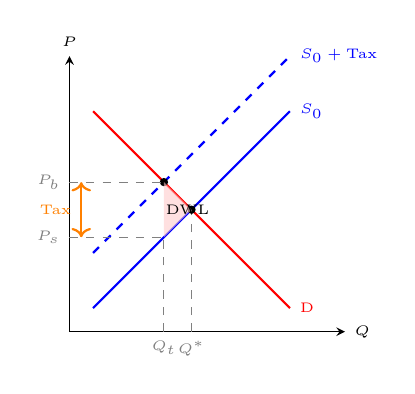
\begin{tikzpicture}[baseline]
    \draw[axis] (0,0) -- (3.5,0) node[right] {$Q$};
    \draw[axis] (0,0) -- (0,3.5) node[above] {$P$};
    % Original S and D
    \draw[thick, blue] (0.3,0.3) -- (2.8,2.8) node[right] {$S_0$};
    \draw[thick, blue, dashed] (0.3,1.0) -- (2.8,3.5) node[right] {$S_0+\text{Tax}$};
    \draw[thick, red] (0.3,2.8) -- (2.8,0.3) node[right] {D};
    % Old eq
    \fill (1.55,1.55) circle (1.5pt);
    \draw[dashed_line] (1.55,0) -- (1.55,1.55) node[below, at start] {$Q^*$};
    % New eq
    \fill (1.2,1.9) circle (1.5pt);
    \draw[dashed_line] (1.2,0) -- (1.2,1.2) node[below, at start] {$Q_t$};
    % Buyer and seller price
    \draw[dashed_line] (0,1.9) -- (1.2,1.9) node[left, at start] {$P_b$};
    \draw[dashed_line] (0,1.2) -- (1.2,1.2) node[left, at start] {$P_s$};
    % Tax wedge
    \draw[<->, thick, orange] (0.15,1.2) -- (0.15,1.9) node[midway, left] {Tax};
    % DWL
    \fill[red!20, opacity=0.6] (1.55,1.55) -- (1.2,1.9) -- (1.2,1.2) -- cycle;
    \node at (1.5,1.55) {DWL};
\end{tikzpicture}
}
\end{center}
\vspace{-5pt}
\begin{itemize}
    \item Tax creates wedge: Buyer pays $P_b$, seller gets $P_s = P_b - \text{Tax}$.
    \item \textbf{Inelastic side bears more burden} (can't escape).
    \item $Q$ falls from $Q^*$ to $Q_t$. DWL = triangle between old and new $Q$.
\end{itemize}

\subsection*{Arc (Midpoint) Elasticity}
$$E_d = \frac{\Delta Q / \bar{Q}}{\Delta P / \bar{P}} = \frac{(Q_2-Q_1)/[(Q_1+Q_2)/2]}{(P_2-P_1)/[(P_1+P_2)/2]}$$
Use midpoint to avoid direction-dependence.

\subsection*{Cross-Price Calc Example}
$E_{xy} = 1.2$ (Coke \& Pepsi). Coke $P \uparrow 10\%$:\\
$\%\Delta Q_{Pepsi} = 1.2 \times 10\% = 12\%\uparrow$.\\
$E_{xy} > 0 \to$ Substitutes. Coke expensive $\to$ buy Pepsi.

$E_{xy} = -0.5$ (physician \& hospital). Physician $P \downarrow$:\\
$\%\Delta Q_{hosp} = -0.5 \times (\text{neg}) = \text{positive} \to$ D Right.\\
$E_{xy} < 0 \to$ Complements. Cheaper doctor $\to$ more hospital use.

\end{multicols*}
\end{document}
